\section{Simulation of the effect of the tourism on the contagion of HPV in Spain}
In $2017$, $82$ millions of tourists visited Spain \cite{INEturismo}. These visits may have influence on the spread of HPV and this is what we are going to study in the present section.

Unfortunately, there are not available data related to the number of infections due to sexual intercourses with tourists, therefore, we are going to introduce a more or less believable scenario, skewing a bit against the vaccine. This scenario will simulate, every month, that $1\%$ of Spanish individuals aged $18-29$ years old with $4$ or more LSP have sexual intercourses with infected tourists.

To do so, we need to introduce a new feature in the computational model to simulate the effect of the tourism. First, recall that, following \cite{castellsague2012prevalence}, among the infected women, $76.03\%$ of them are infected of HPV HR, $11.72\%$ are infected of HPV LR and $12.24\%$ are infected by both, HR and LR. Also, $50.35\%$ of the HPV HR are with oncogenic types, that is, HPV 16/18/31/33/45/52/58. Furthermore, $37.075\%$ of the HPV LR are with 6/11. Then, for all individuals with $4$ or more LSP aged $18-29$ ($rnd()$ denotes a computational function that generates a random number in the interval $[0,1]$.

\begin{itemize}
	\item If $rnd()<0.01$ (the individual may be infected by a tourist) and let $x=rnd()$
	\begin{itemize}
		\item If $x < 0.7603$ the node gets infected by HPV HR. Also, if $rnd() < 0.5035$ and the individual is not vaccinated, the infection is by an oncogenic HPV HR.
		\item If $0.7603 \leq x < 0.7603 + 0.1172$ the node gets infected by HPV LR. Also, if $rnd() < 0.3707$ and the individual is not vaccinated, the infection is by HPV 6/11.
		\item If $0.7603 + 0.1172 \leq x $ the node gets infected by HPV LR and by HPV LR (coinfection). Thus, if $rnd() < 0.5035$ and the individual is not vaccinated, the infection is by an oncogenic HPV HR and $rnd() < 0.3707$ the infection is also by HPV 6/11.
	\end{itemize}
\end{itemize}

Including the above features in the computational model and performing a simulation, in the Figure \ref{fig:turismo} we can see the influence of the tourism in the HPV infections.

\begin{figure}[!]
	\centering
	\begin{tabular}{cc}
		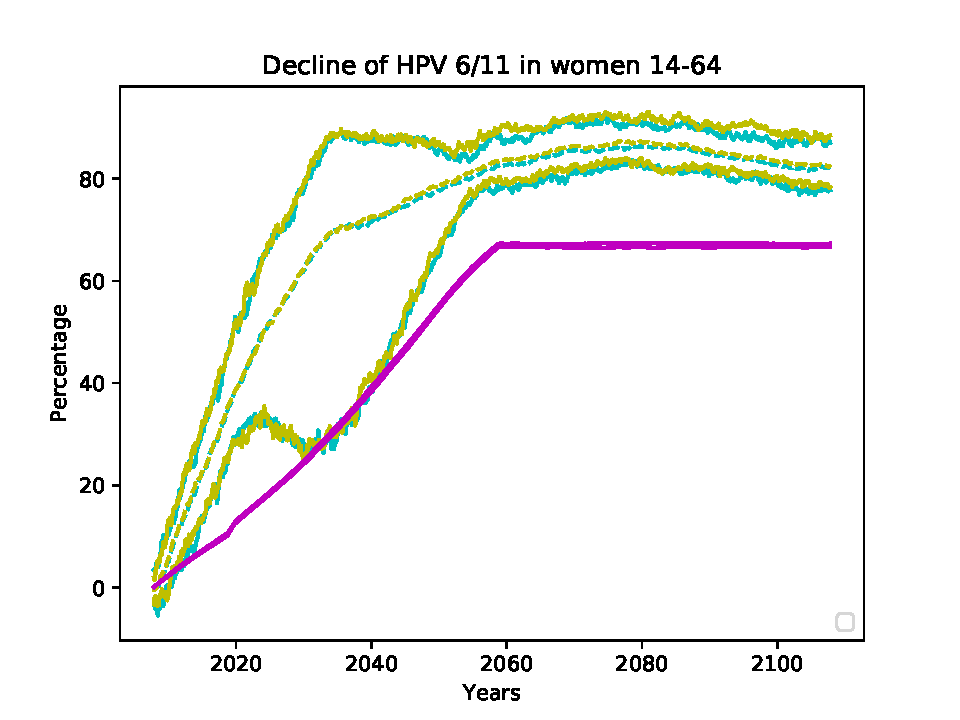
\includegraphics[width=0.5\linewidth]{IMGs/8.-Turismo/verr_muj.pdf}	& 
		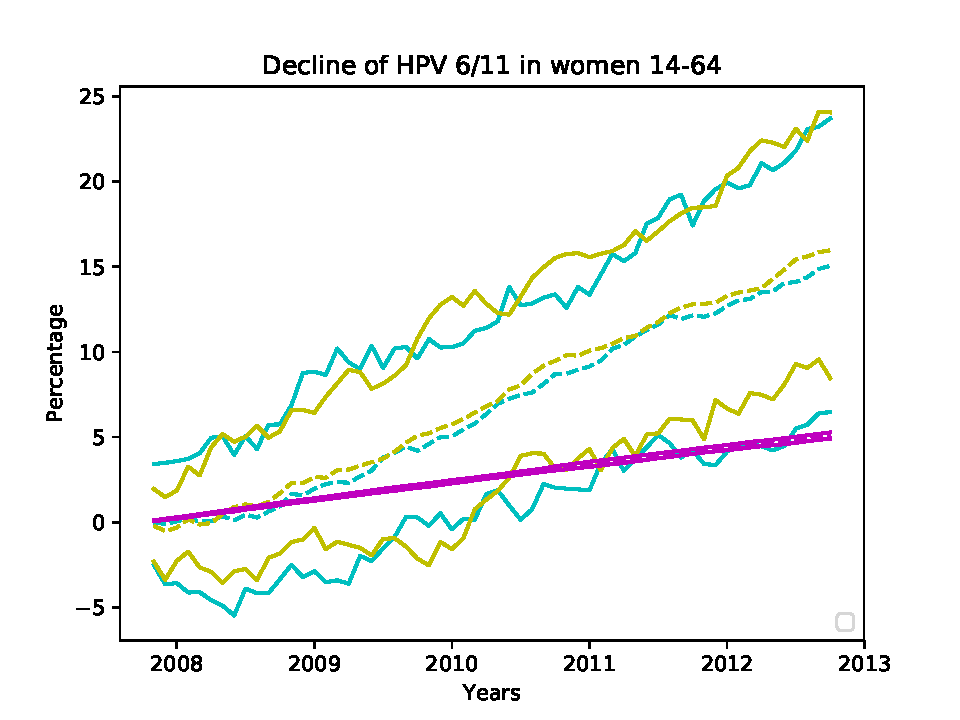
\includegraphics[width=0.5\linewidth]{IMGs/8.-Turismo/verr_muj_ZOOM.pdf}  \\ 
		(a)	& (b) \\ 
		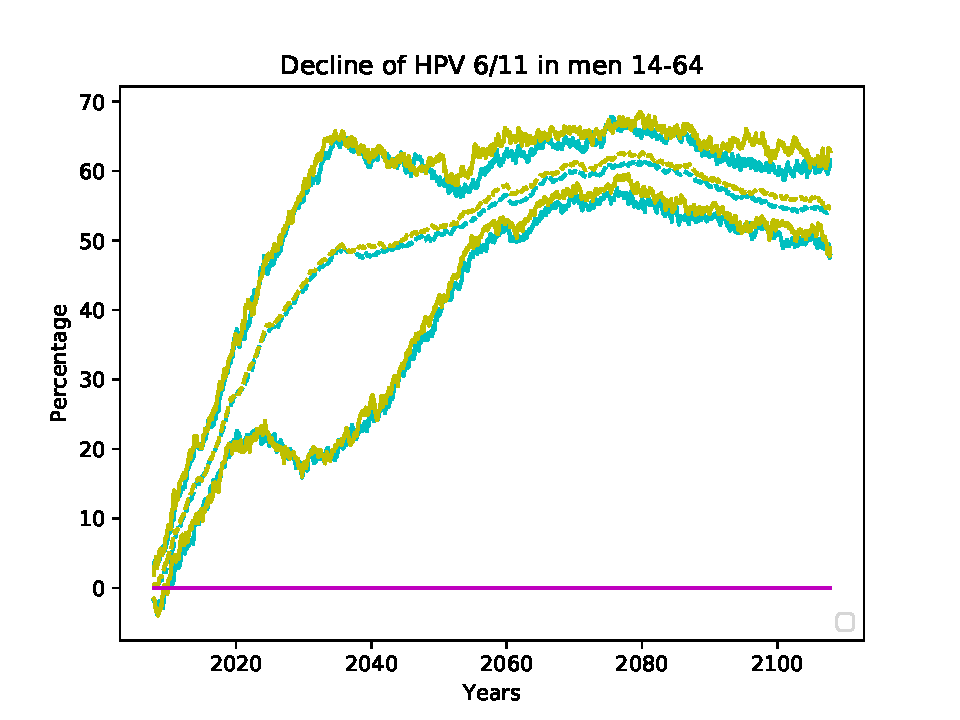
\includegraphics[width=0.5\linewidth]{IMGs/8.-Turismo/verr_hom.pdf}	& 
		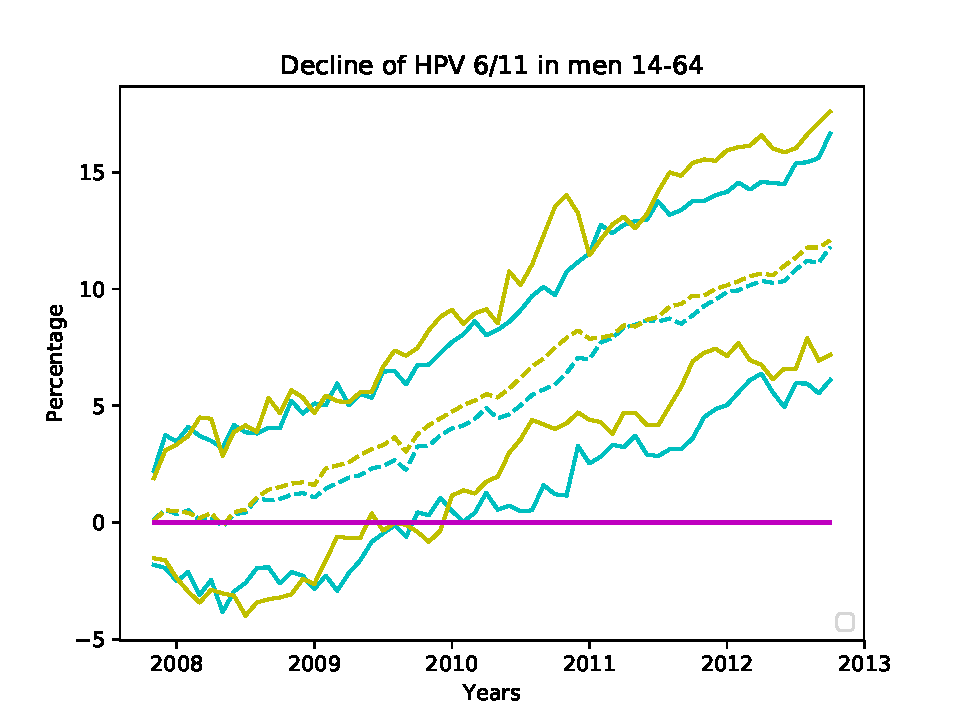
\includegraphics[width=0.5\linewidth]{IMGs/8.-Turismo/verr_hom_ZOOM.pdf}  \\ 
		(c)	& (d) \\ 		
		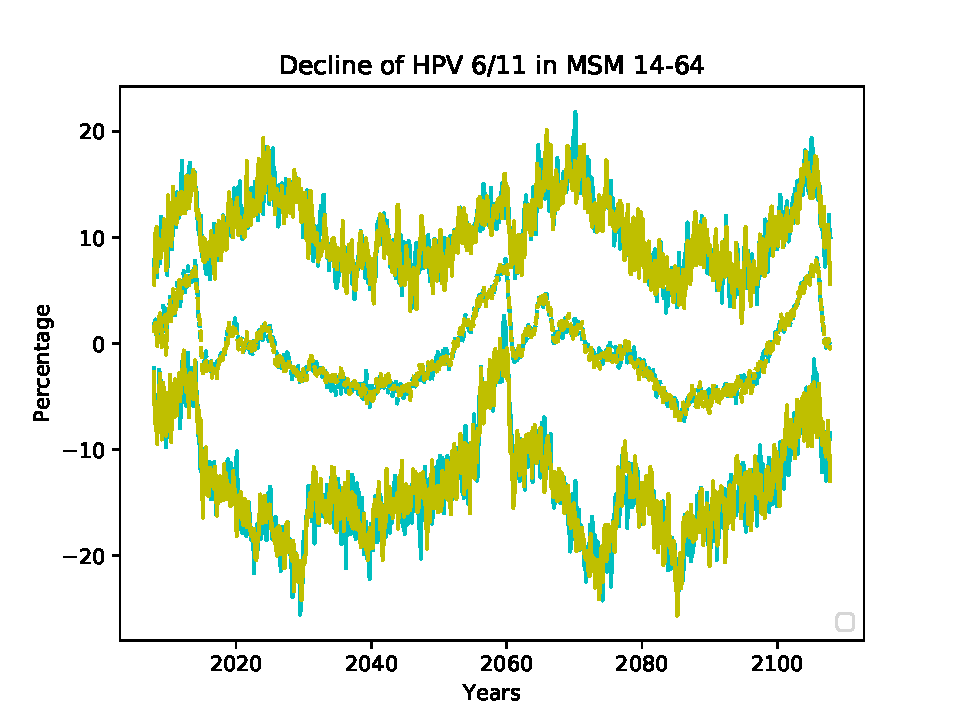
\includegraphics[width=0.5\linewidth]{IMGs/8.-Turismo/verr_MSM.pdf}	& 
		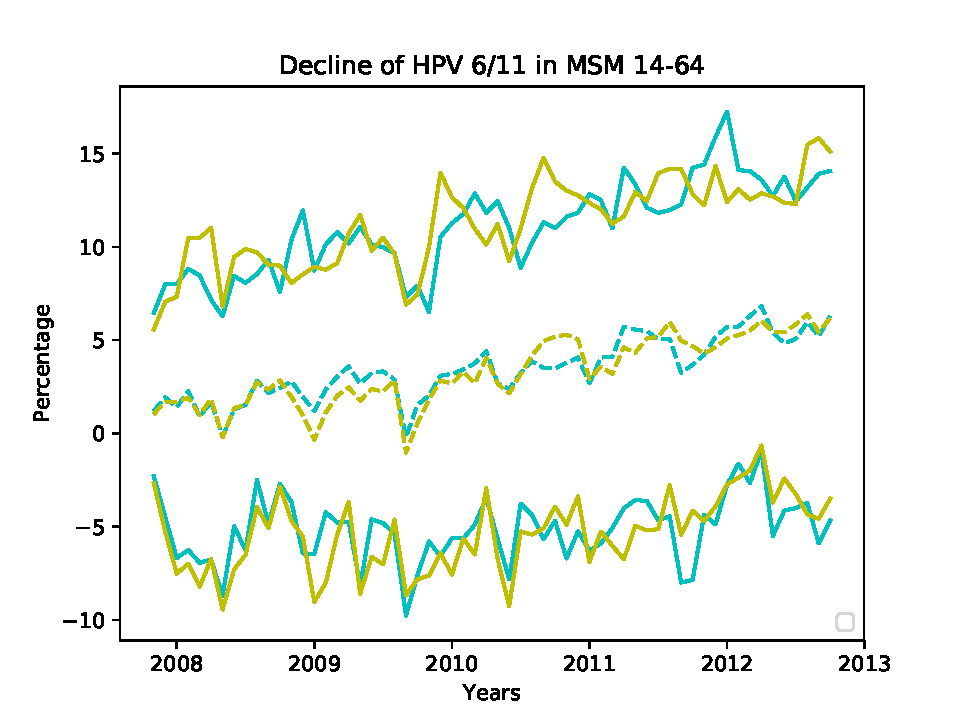
\includegraphics[width=0.5\linewidth]{IMGs/8.-Turismo/verr_MSM_ZOOM.pdf}  \\ 
		(e)	& (f)
 	\end{tabular} 
	\caption{Comparative of the decline of  HPV LR 6/11 in 14-64 years old women (a), men (c) and MSM (e) over the time and a zoom of the graphs for the first five years for women (b), men (d) and MSM (f), between the non-tourism scenario (yellow lines) and the tourism scenario where every month $1\%$ of Spanish individuals aged $18-29$ years old with $4$ or more LSP have sexual intercourses with infected tourists (cyan lines). Magenta lines show the percentage of vaccinate women and men (nobody in men). No remarkable changes appear.}
	\label{fig:turismo}
\end{figure}

Figure \ref{fig:turismo} shows that there are not remarkable differences between both scenarios including the very beginning, where there are very few girls vaccinated. Therefore, the tourism does not seem to be a factor that influences the decline the HPV 6/11. Here we do not show the same graphs for HPV oncogenic because of their similarity with the ones in Figure \ref{fig:turismo}. 
